% 3장 자료와 시스템. CS 기여. 8~10쪽.
% 쓰는 방식: "무엇을 만들었다" 가 아니라 "그게 없었으면 2층이 불가능했다".

\section{자료와 시스템}

제목의 1층이 이 장이다. 다만 \textbf{잘게 쪼갠 것 자체는 기여가 아니다.} 의의는
\textbf{미시 자료가 아니면 보이지 않는 것을 실제로 보였다}는 데 있다. 이 장의
각 절은 그 대응 관계를 밝히는 순서로 쓴다.

\begin{table}[htbp]
  \centering
  \caption{미시 자료가 아니면 보이지 않는 것}
  \label{tab:micro-need}
  \begin{tabular}{p{5.2cm}p{4.0cm}p{5.0cm}}
    \toprule
    \textbf{발견} & \textbf{필요했던 미시 정보} & \textbf{동 단위 집계로는} \\
    \midrule
    직후 효과 $-59\% \to -76\%$ & 거래 하나하나의 \textbf{계약일} &
      달력 월 안에서 지정 전후를 못 가른다 \\
    공고와 효력 사이 나흘의 막차 수요 & 하루 단위 거래 & 안 보인다 \\
    면적 기준이 회피 통로 & 거래마다의 \textbf{전용면적} &
      동 전체 거래 수만 있어 불가능 \\
    중위가가 11포인트 부풀려짐 & \textbf{같은 집}의 반복 거래 &
      구성 변화를 못 걷어낸다 \\
    2025년 부분 해제 & \textbf{단지}별 해제·유지 여부 &
      같은 동 안의 두 집단을 못 가른다 \\
    `인근 급등'이 기준점의 산물 & 서울 전역 단지를 \textbf{한 표}에 &
      처치동 인근만 보게 되어 기준점을 못 옮긴다 \\
    두 사건을 \textbf{같은 자}로 & 서울 25개 구를 하나의 패널로 &
      사건마다 통제군이 달라져 차이를 못 잰다 \\
    \bottomrule
  \end{tabular}
\end{table}

선행연구가 동 단위 집계로 ``60\% 줄었다''에서 멈춘 이유가 여기 있다. 그 이상으로
나아갈 정보가 자료에 없었다.

\subsection{실거래 상세 자료}

국토교통부가 공개하는 아파트 매매 실거래 자료는 두 종류다. 일반 자료와
\textbf{상세 자료}(\texttt{RTMSDataSvcAptTradeDev})이며 활용신청이 개별적으로
필요하다. 상세 자료라야 \texttt{aptSeq}(단지 식별자), \texttt{excluUseAr}
(전용면적), \texttt{floor}(층), \texttt{buildYear}(건축연도), 그리고 계약
\textbf{일자}가 함께 온다.

정제를 마친 표본은 표 \ref{tab:sample}과 같다. \textbf{같은 자료를 두 장으로
짓는다} --- 분석 8개 자치구와 서울 25개 자치구다. 뒤쪽이 필요한 이유는 통제군에
있다. 합성대조군은 처치동과 비슷한 동을 서울 전역에서 찾아야 하고(9.2절),
2021년 B그룹은 영등포·양천·성동구까지 걸쳐 있어 8개 구 안에 통제군이 없다
(9.6절). \textbf{기준점을 옮겨 가며 파급을 재는 것}도 서울 전역 패널이라야
가능하다(7.3절).

% 자동 생성 — scripts/build_tables.py. 손으로 고치지 않는다.
% 출처: output/results/02_build.json
\begin{table}[htbp]
  \centering
  \caption{표본 요약. 두 장을 함께 짓는 이유는 \textbf{통제군}에 있다 --- 합성대조군의 기증자 풀과 2021년 B그룹 분석이 서울 전역 패널을 쓴다.}
  \label{tab:sample}
  \begin{tabular}{lrr}
    \toprule
    \textbf{} & \textbf{분석 8개 자치구} & \textbf{서울 25개 자치구} \\
    \midrule
    거래 (건) & 472,782 & 1,407,186 \\
    단지 (aptSeq) & 3,502 & 9,240 \\
    법정동 & 108 & 343 \\
    자치구 & 8 & 25 \\
    반복매매 쌍 & 377,289 & 1,158,318 \\
    제외 --- 취소거래 & 6,293 & 17,307 \\
    제외 --- 신고지연 절단 & 3,156 & 13,677 \\
    계약일 구간 & 2006-01-02 \textasciitilde{} 2026-05-31 & 2006-01-01 \textasciitilde{} 2026-05-31 \\
    수집 시점 & 2026-09-03 & 2026-09-03 \\
    \bottomrule
  \end{tabular}

  \begin{minipage}{\linewidth}\footnotesize
  \textit{주.} 같은 스냅샷에서 같은 규칙으로 정제했다. 분석 패널은 8개 자치구(강남·서초·송파·강동·성동·광진·동작·용산), 서울 패널은 25개 자치구 전체다. 반복매매 쌍은 (단지, 전용면적, 층) 조합의 재거래이며 보유 180일 미만을 뺀 수다(0018).
  \end{minipage}
\end{table}


단지 식별자가 왜 결정적인지는 간단한 예로 알 수 있다. 어느 동에서 한 달에
100건이 팔리다가 20건으로 줄었다고 하자. 줄어드는 비율이 단지마다 다르면
\textbf{각 단지의 가격이 하나도 변하지 않아도 동 평균은 움직인다.} 측정된
``평균 가격 변화'' 안에 진짜 가격 변화와 구성 변화가 섞인다. 실제로 처치동
사후 표본의 평균 전용면적이 93.9\,m$^2$에서 88.7\,m$^2$로 이동했다.

사양 12개를 비교해 보면 \textbf{단위 고정효과 수준이 결과 크기를 두 배 갈랐다}
(0003). 법정동 수준에서 비교하면 가격 효과가 $-12.3 \sim -15.8\%$, 단지 수준으로
내리면 $-6.0 \sim -8.0\%$다. 창 길이($\pm$12/24/36개월)와 통제군 범위(2개 구/8개
구)는 거의 영향이 없었다. \textbf{결과를 좌우하는 유일한 설계 선택이 단위
고정효과였다.}

\subsection{공고 원문에서 법정동 패널까지}

토허구역의 ``어디가 언제''는 공고에만 있다. 그래서 공고를 자료로 다룬다.

\begin{enumerate}[leftmargin=2em, itemsep=2pt]
  \item \textbf{원문 수집.} 서울시보와 전자관보에서 지정·재지정·해제 공고를
        모은다. 서울시보 원본은 2.9\,GB라 저장소 밖에 두고, 발췌한 PDF만 넣는다.
  \item \textbf{본문 텍스트 추출.} PDF에서 글자를 뽑되, 글꼴마다 한글 코드가
        다르게 매핑되는 문제를 글꼴별 오프셋으로 교정한다
        (\texttt{lib/pdftext.py}).
  \item \textbf{구역 표 추출.} 공고 별표에서 자치구·법정동·지번·면적 기준을
        읽는다. 판독 건수는 현재 1,168건이다.
  \item \textbf{지정 구간 생성.} 같은 법정동의 공고들을 시간 순으로 이어 붙여
        \texttt{[시작일, 종료일)} 구간으로 만든다.
  \item \textbf{거래에 결합.} 거래의 계약일과 법정동으로 그 시점의 규제 상태를
        붙인다.
\end{enumerate}

여기서 두 가지 판단이 필요했다.

\textbf{(가) 지정 범위를 동 전체로 볼 것인가}(0010). 공고는 지번 단위로 적는
경우와 동 전체로 적는 경우가 섞여 있다. 2020년 6월 공고는 네 개 동을 동 전체로
지정했음을 지형도면으로 확인했다. 확인 과정에서 외부 자료가 효력일을
2020-06-19로 답했으나 \textbf{공고 2020-1832호 원문은 2020-06-23}이었다. 원문을
따랐다. 2차 자료의 한계를 보여 주는 사례다.

\textbf{(나) 유지 단지를 어떻게 확정할 것인가}(0008). 2025년 2월 부분 해제에서
지정이 유지된 단지를 단지명으로 맞추면 자료마다 14개, 13개, 15개로 갈렸다.
공고 제2025-497호 별표의 \textbf{지번}으로 매칭해 실거래 자료의
\textbf{16개 단지 식별자}로 확정했다(선경이 1차·2차로, 한보미도맨션이 1·2로
나뉜다).

\textbf{(다) 통제군 오염 점검}(0009, 0020). 통제군에 있어야 할 동이 나중에
토허구역으로 지정되면 처치·통제 격차가 줄어 추정치가 0 쪽으로 끌린다. 강남·송파
통제동 23개 가운데 여섯(거여·압구정·마천·송파·신천·일원)이 분석 창 안에서
지정됐음을 찾았고, \textbf{제외 목록을 결과를 보기 전(2026-09-07)에 확정}한 뒤
분석했다(9.3절).

\subsection{표본 정제}

정제 규칙은 둘이다(0004).

\textbf{취소거래 제외.} \texttt{cdealType}이 \texttt{'O'}인 해제 거래를 뺀다.
8개 자치구·2026-09-03 수집 기준 원자료 482,231건 중 6,293건(1.30\%)이다. 신고 후
취소되는 거래에는 시세 조작 목적의 허위 신고가 섞일 수 있고, 규제 시점 전후로
몰리면 추정치를 위로 편향시킨다.

\textbf{신고지연 절단.} 신고기한이 계약일로부터 30일이라 수집 시점에 가까운
계약월은 신고가 덜 들어와 과소집계된다. 2026-05에서 06으로 넘어가며 거래가 절반
이하로 떨어지므로 보수적으로 \textbf{2026-05까지만} 쓴다. 신고율을 추정해
역산하는 방법도 있으나 그 추정의 불확실성을 자료에 섞어 넣게 되므로 버리는 쪽을
택했다.

이 연구에는 \textbf{절단이 둘}이고 섞이기 쉬우므로 분명히 둔다. 자료 품질 때문에
표본 끝을 2026-05-31에서 끊고(0004), 통제군 소멸 때문에 인과추정을
2025-10-19에서 끊는다(0002). \textbf{뒤쪽이 더 강한 제약}이므로 신고지연 절단은
실제로 인과추정에 영향을 주지 않는다.

\textbf{뺀 것이 결과를 바꾸는지 확인했다}(0030). 취소거래를 다시 넣어 같은 사양을
돌리면 지정 직후 효과가 $-79.8\%$에서 $-79.5\%$로 \textbf{0.3\,\%p} 움직인다.
규제 직후에 몰리지도 않는다 --- 세 사건에 대해 취소율의 이중차분이 창에 따라
$-2.3 \sim +1.7$\,\%p로 부호가 바뀐다(9.7절).

\subsection{자체 가격지수}

거래가 80\% 줄면 팔리는 물건의 구성이 바뀌므로, 가격을 해석하려면 구성 변화를
걷어내야 한다. 약점이 \textbf{정반대}인 두 방법을 모두 지었다.

\textbf{반복매매지수}(0018)는 같은 물건의 두 거래만 쓴다. 같은 집이면 면적·층·
단지·입지가 전부 같으므로 구성이 원천적으로 바뀔 수 없다. 추정식은
\[
\log P_{t_2} - \log P_{t_1} = \beta_{t_2} - \beta_{t_1} + \varepsilon
\]
이고, $t_2$에 $+1$ · $t_1$에 $-1$인 희소 행렬로 회귀한다
\citep{bailey1963regression}. 오래 보유한 쌍일수록 가격 변화의 분산이 커지므로
\citet{caseshiller1987}의 3단계 가중을 쓴다 --- 잔차 제곱을 보유기간에 회귀하고
그 역수의 제곱근으로 다시 추정한다. 실측 기울기가 보유 1년당 분산 $+0.006$으로
가정과 맞았다.

세 가지를 정했다. 첫째, 실거래 자료에 \textbf{호실 번호가 없으므로} 물건을
(단지, 전용면적, 층)으로 본다. 월 단위로 5.8\%의 칸에 두 건 이상이 들어가지만,
같은 단지·면적·층이면 가격이 거의 같아 서로 바뀌어 짝지어져도 편의가 2차적이다.
둘째, \textbf{보유 180일 미만을 뺀다} --- `가격 변화가 정확히 0'인 쌍의 비중이
4.1\%에서 1.5\%로 떨어지고 그 뒤로는 완만하다. 셋째, 연율 로그수익률 $\pm$50\%
초과를 뺀다(전체의 0.5\%).

\textbf{헤도닉 지수}(0025)는 반대로 모든 거래를 쓰되 특성을 통제한다.
\[
\log(\text{㎡당가}) \sim \text{월 더미} + \log(\text{면적}) +
\log(\text{면적})^2 + \text{층 구간 더미}
\]
월 더미가 지수다. \textbf{연식은 넣지 않는다} --- 단지 고정효과 아래에서 연식은
시간의 일차함수라 월 더미에 완전히 흡수된다(제거 후 잔차 $10^{-10}$). 넣어도
계수는 같지만 읽는 사람이 통제된 줄로 오해한다.

% 자동 생성 — scripts/build_tables.py. 손으로 고치지 않는다.
% 출처: output/results/08_hedonic.json : 지수_사다리
\begin{table}[htbp]
  \centering
  \caption{구성 통제의 사다리. 아래로 갈수록 더 많은 것을 고정한다.}
  \label{tab:index-ladder}
  \begin{tabular}{lrrr}
    \toprule
    \textbf{가격지수} & \textbf{지정 전 비} & \textbf{지정 후 비} & \textbf{변화 (\%)} \\
    \midrule
    중위가(총액) & 0.945 & 0.849 & -10.1 \\
    중위가(㎡당) & 1.012 & 0.885 & -12.5 \\
    헤도닉 & 0.979 & 0.870 & -11.1 \\
    헤도닉+단지 & 0.985 & 0.927 & -5.9 \\
    반복매매 & 1.001 & 0.941 & -6.0 \\
    \bottomrule
  \end{tabular}

  \begin{minipage}{\linewidth}\footnotesize
  \textit{주.} 약점이 정반대인 두 방법(헤도닉과 반복매매)이 $-5.9\%$ 와 $-6.0\%$ 에서 만난다. 집계 지수의 $-10 \sim -12\%$ 는 절반쯤이 구성 변화였다.
  \end{minipage}
\end{table}


\begin{figure}[htbp]
  \centering
  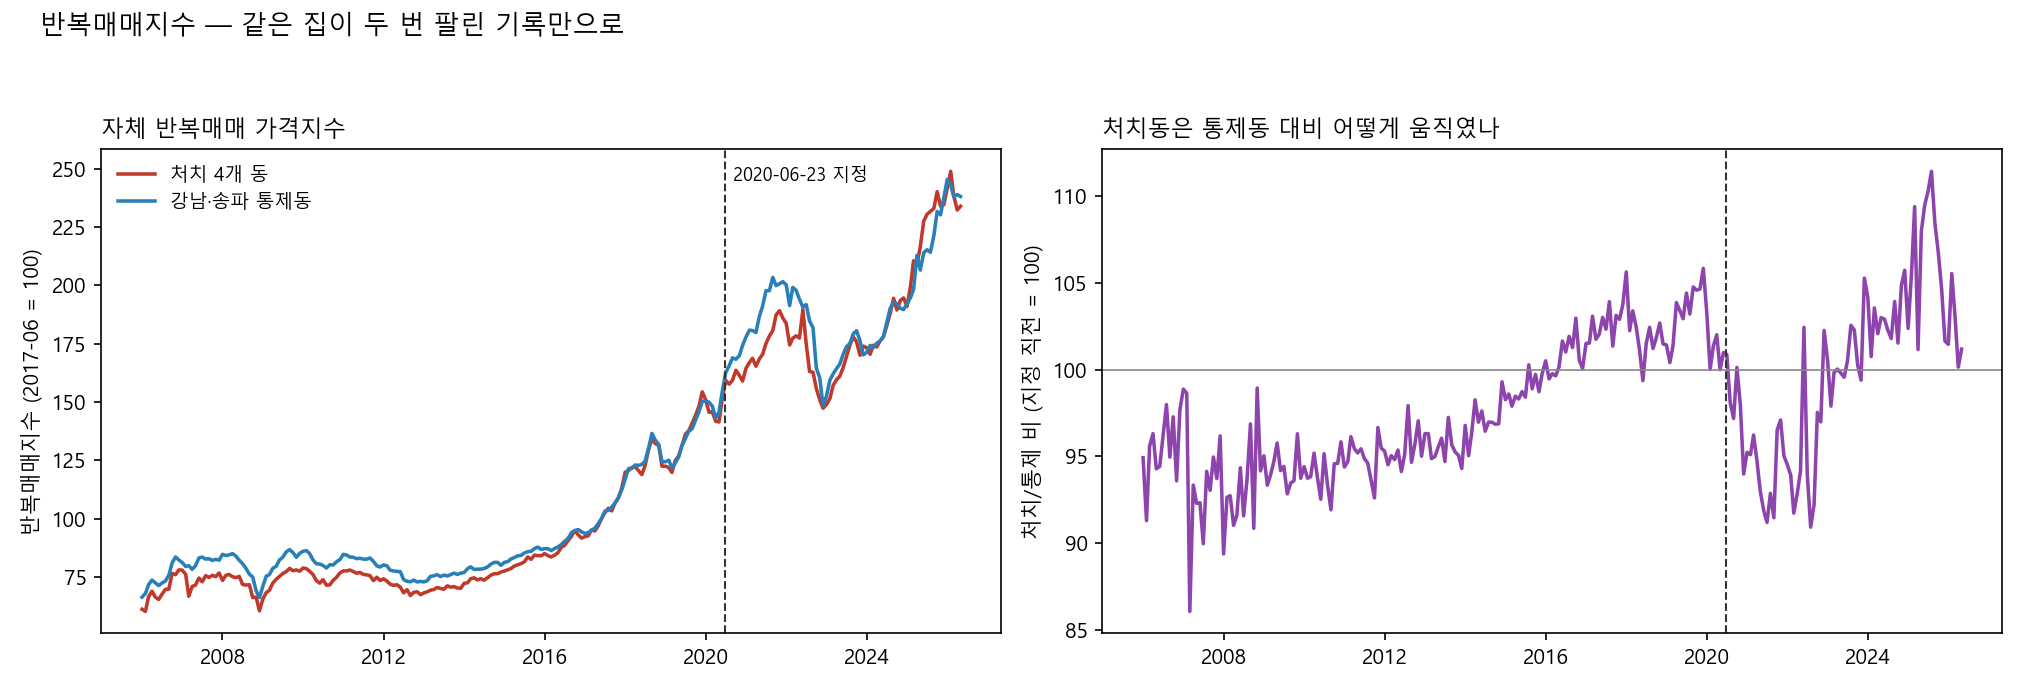
\includegraphics[width=\linewidth]{07_repeat_sales.png}
  \caption{반복매매 가격지수. 2017-06 = 100.}
  \label{fig:repeat-sales}
\end{figure}

\textbf{약점이 정반대인 두 방법이 $-5.9\%$와 $-6.0\%$에서 만난다.} 반복매매는 두
번 팔린 집만 쓰고(선택편의), 헤도닉은 관측되는 특성만 통제한다. 둘이 일치하면
서로를 떠받친다. 그리고 집계 지수의 $-10 \sim -12\%$는 \textbf{절반쯤이 구성
변화}였음을 보여 준다.

지수 자체의 그럴듯함도 확인했다. 2017-06을 100으로 두면 2021-06에 187,
2022-06에 190, 2023-06에 169($-11\%$), 2026-05에 237이다. 2022년 금리 급등기의
조정과 이후 재상승이 그대로 나타난다.

\subsection{재현 장치}

\textbf{이 절이 이 보고서에서 가장 `시스템'다운 부분이다.} 숫자가 아니라
\textbf{숫자를 믿게 만드는 장치}를 지었다는 이야기다.

원자료 수집부터 그림·표 생성까지 \textbf{\pipeSteps 단계 파이프라인} 하나로 돈다
(\texttt{python run\_all.py}). 단계는 자료 \pipeData, 정책 \pipePolicy, 분석
\pipeAnalysis, 재현 \pipeReplicate, 시각화 \pipeViz, 문서 \pipeDocs 로 나뉘고,
뒤 단계가 앞 단계 산출물을 읽으므로 하나라도 실패하면 거기서 멈춘다. 그림
\ref{fig:pipeline}이 전체 흐름이다.

\textbf{이 문단의 단계 수도 손으로 적지 않았다.} 주차 보고서가 한 편 늘면 문서
단계가 하나 늘기 때문에, 손으로 적으면 그 순간 틀린 값이 된다. 도식을 그리는
스크립트가 \texttt{run\_all.py}의 단계 표를 읽어 세고 그 값을 매크로로 내보낸다.

\begin{figure}[htbp]
  \centering
  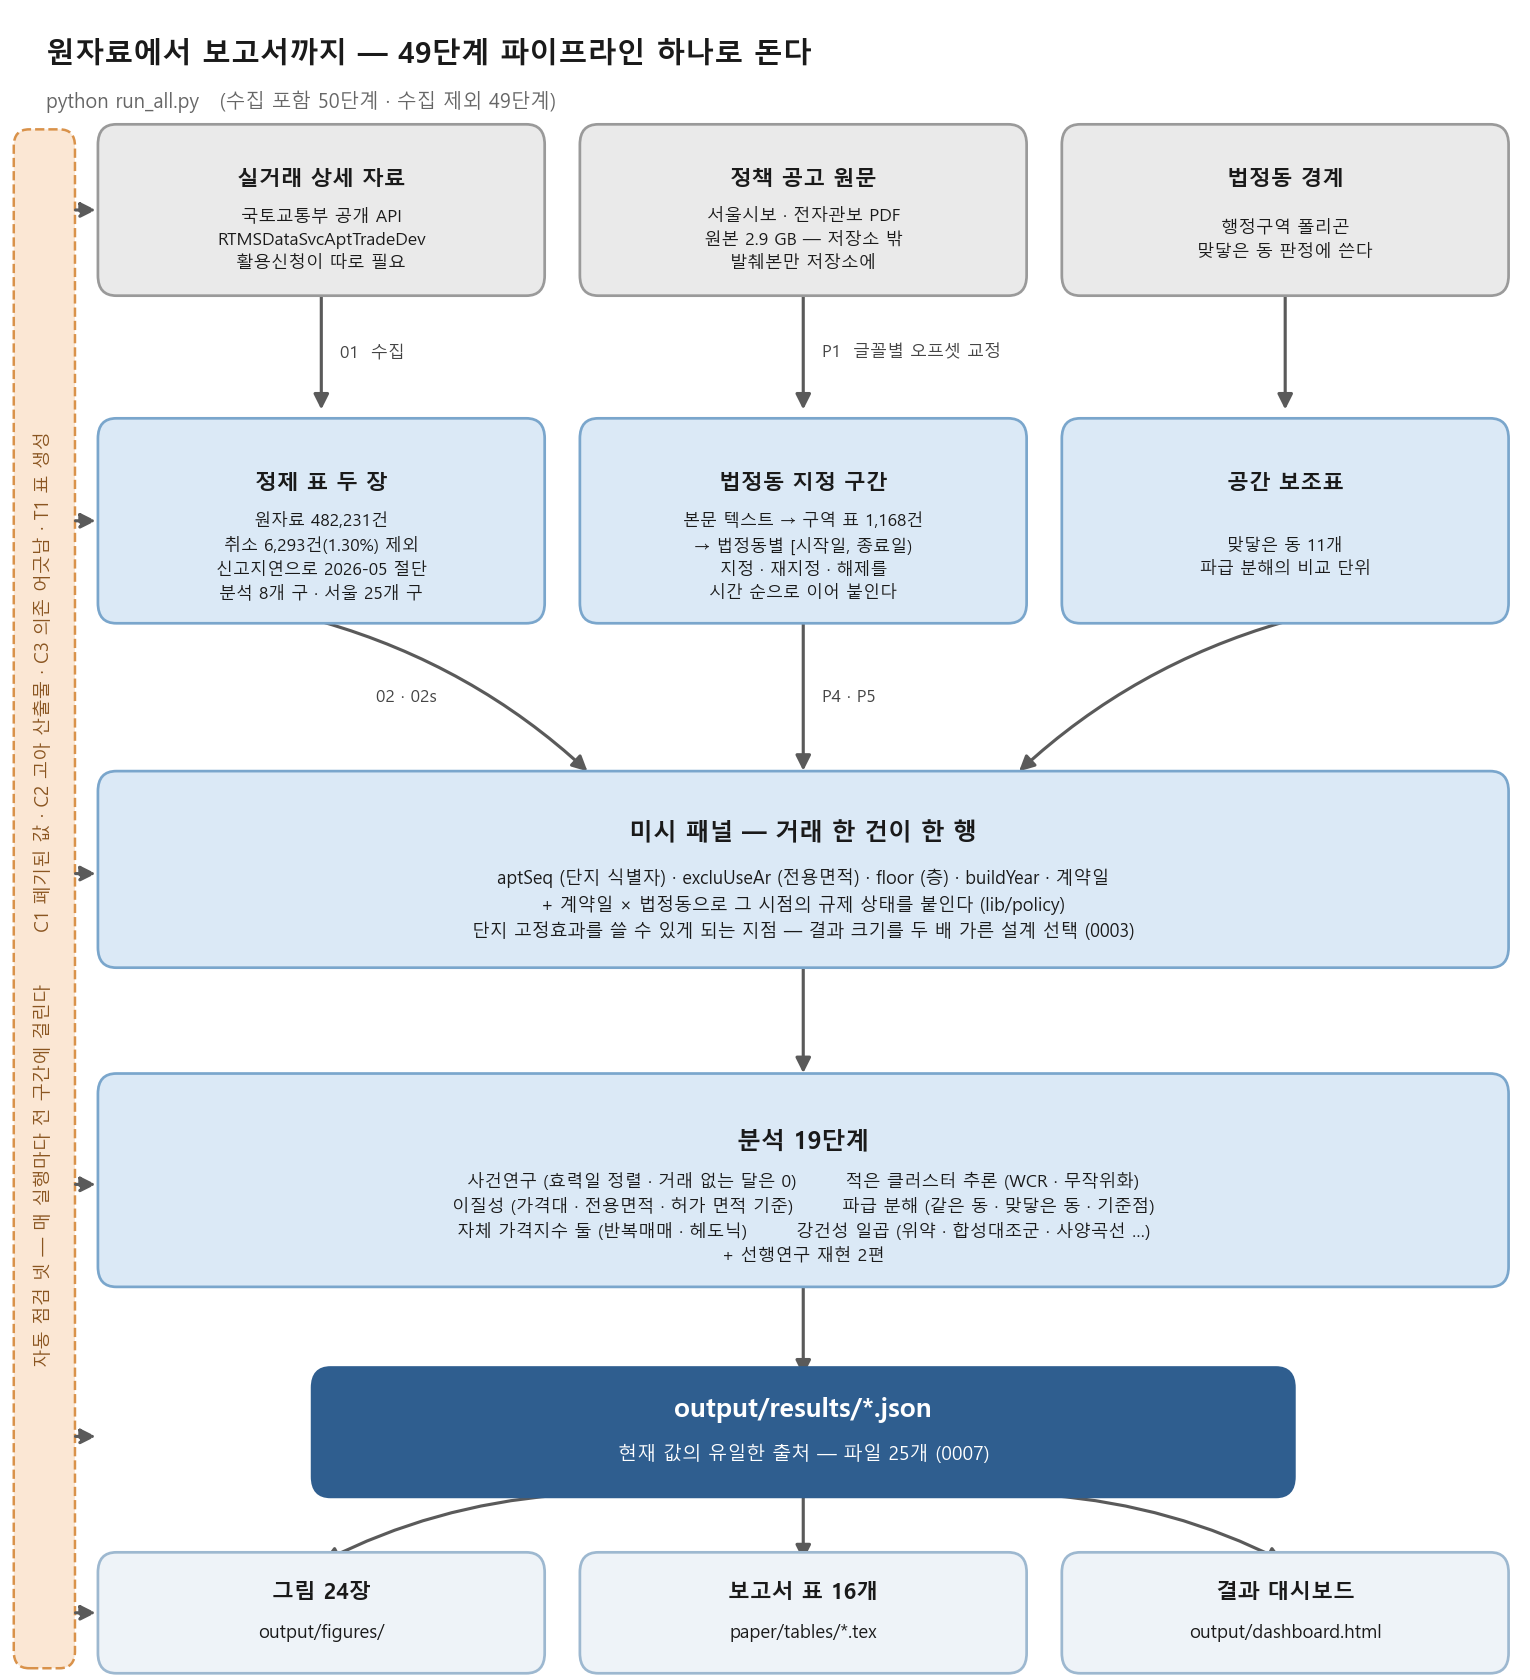
\includegraphics[height=0.86\textheight]{pipeline.png}
  \caption[원자료에서 보고서까지 --- \pipeSteps 단계 파이프라인]{%
    원자료에서 보고서까지. 입구는 셋이지만 \textbf{출구는 하나}다 ---
    현재 값의 출처는 \texttt{output/results/*.json} 하나이며(0007), 보고서의 표와
    결과 대시보드는 거기서 생성된다. 가운데 줄기(공고 PDF $\to$ 법정동 지정
    구간)가 없으면 처치 변수 자체가 없다. 왼쪽 띠의 점검 넷은 분석 뒤가 아니라
    매 실행마다 걸린다. \textbf{이 그림의 숫자도 손으로 적은 것이 아니라
    \texttt{run\_all.py}와 산출물 폴더를 센 것이다.}}
  \label{fig:pipeline}
\end{figure}

그 위에 점검 넷이 매 실행마다 걸린다.

\begin{table}[htbp]
  \centering
  \caption{자동 점검 넷}
  \label{tab:checks}
  \begin{tabular}{llp{7.5cm}}
    \toprule
    \textbf{단계} & \textbf{스크립트} & \textbf{무엇을 잡나} \\
    \midrule
    C1 & \texttt{check\_numbers.py} &
      살아있는 문서와 결정기록에 남은 \textbf{폐기된 값}.
      조건이 붙은 줄은 통과시킨다 \\
    C2 & \texttt{check\_stale.py} &
      이번 실행에서 \textbf{다시 만들어지지 않은} 산출물,
      그리고 만들어 놓고 \textbf{아무도 가리키지 않는} 문서 \\
    C3 & \texttt{check\_deps.py} &
      \texttt{requirements.txt}와 실제 import의 어긋남.
      함수 안의 늦은 import까지 AST로 훑는다 \\
    T1 & \texttt{build\_tables.py} &
      보고서의 표를 결과 JSON에서 생성. 가리키는 키가 없으면 알린다 \\
    \bottomrule
  \end{tabular}
\end{table}

설계 원칙은 하나다. \textbf{현재 값의 출처는 \texttt{output/results/*.json}
하나다}(0007). 문서의 숫자가 이 파일과 어긋나면 JSON이 맞다. 그래서 보고서의
표와 결과 대시보드는 \textbf{숫자를 손으로 적지 않는다} --- 적는 것은 ``어디서
꺼낼지''와 ``어떻게 보일지''뿐이다.

문서는 세 종류로 나눈다. \textbf{동결}(주차 보고서·발표 자료)은 그 시점의
기록이므로 갱신하지 않고, \textbf{살아있는}(백로그·용어집·연구의 뼈대)은 항상
현재 상태이며, \textbf{최종}(이 보고서)은 하나의 조건으로 통일한다. 다만 동결
문서라도 \textbf{작성 시점에 이미 틀린 값}은 정정하고 그 사실을 남긴다.

\subsection{클린 환경 재현}

장치가 돈다는 말을 하려면 \textbf{받는 사람의 환경}에서 확인해야 한다. 새 폴더에
내려받아 새 가상환경에서 돌렸다.

\textbf{멈췄다.} 12단계에서 \texttt{shapely}를 찾지 못했다.
\texttt{requirements.txt}에 \texttt{shapely}와 \texttt{markdown}이 빠져
있었던 것이다. 법정동 경계로 맞닿은 동을 찾을 때와 보고서 HTML을 만들 때 쓰는데,
작업 환경에는 다른 경로로 깔려 있어 몇 주 동안 드러나지 않았다.
\textbf{받는 사람만 겪고 만드는 사람은 못 보는 고장}이다.

고친 뒤 전 단계가 돌았고(약 21분) \textbf{\texttt{output/results/*.json} 25개가
바이트 단위로 같았다.} 그리고 같은 일이 다시 생기지 않도록 \texttt{check\_deps.py}를
만들어 파이프라인에 넣었다.

절차에서 알게 된 것 셋을 \texttt{README}에 적었다. 첫째, \textbf{원자료는
재수집하면 안 된다} --- 실거래 자료는 취소와 지연신고로 소급 갱신되므로 다시
받으면 다른 자료가 온다. 재현은 \textbf{같은 스냅샷 위에서} 하는 것이다. 둘째,
윈도의 경로 길이 한계(260자) 때문에 깊은 폴더에서는 \texttt{statsmodels} 설치가
깨진다. 셋째, 그림을 매번 커밋해 \texttt{.git}이 936\,MB다.

\subsection{유령 숫자 사건}

앞 절의 장치들을 \emph{왜} 만들었는지가 이 절이다.

\texttt{output/results/es\_price.csv}와 \texttt{es\_volume.csv}가 2026-09-03
파일이었다. 그 사이 사건연구 스크립트가 JSON 저장으로 바뀌면서
\textbf{아무도 그 CSV를 만들지 않게 됐다.} 그래서 사건 시점 정렬 수정(0013)
\emph{이전} 숫자($k=0$에서 $-58.7\%$)가 석 달 가까이 남아 있었다.

\textbf{전체 재실행을 두 번 했는데도 못 잡았다.} 전체 재실행은 다시 만들어지는
파일만 본다. 아무도 만들지 않는 파일은 \texttt{git status}에도 뜨지 않고 영원히
낡은 채로 남는다.

그래서 \texttt{check\_stale.py}를 만들었다. 바뀐 것이 아니라 \textbf{안 바뀐
것}을 센다. 붙이자마자 다섯을 더 잡았다. 고아 파일 네 개를 지웠고, 그중
\texttt{current\_zones.csv}에는 유지 단지가 ``14개''로 적혀 있었다 --- 0008에서
16개로 확정한 뒤 폐기된 숫자다. 그리고 결정기록 0004에 \textbf{6개 자치구 시절
값}(4,285건)이 남아 있었다. 결정기록이 검사 대상에서 빠져 있었기 때문에 다섯 달
동안 드러나지 않았다. 검사 대상에 넣은 뒤 \textbf{나머지는 전부 깨끗했다}
(당시 28편, 현재 30편).

\textbf{제목의 두 층이 여기서 만난다.} 1층(미시 패널 구축)은 2층(인과추정)이
답할 수 있게 해 주는 전제이고, 그 전제가 썩지 않게 지키는 것이 이 절의 장치들이다.
제안서가 ``데이터 엔지니어링이 분석의 부속물이 아니라 식별 전략의 전제''라고 쓴
것이 이 뜻이며, 6장의 면적 기준 발견이 그 주장의 가장 좋은 증거다.
